\chapter{Бағытталған граф}

Осы тарауда біз бағытталған графтың екі түрін қарастырамыз:
% In this chapter, we focus on two classes of directed graphs:
\begin{itemize}
\item \key{Циклсіз граф}:
графта ешқандай цикл жоқ, яғни бір төбеден басталып, 
сол төбеден аяқталатын жол болмайды.
% so there is no path from any node to itself.
\item \key{Мирасқорлар графы}:
әр төбенің шығыстың жарты дәрежесі 1-ге тең, 
яғни әр төбенің бірегей мирасқор болады.
% The outdegree of each node is 1,
% so each node has a unique successor.    
\end{itemize}
Екі жағдайда да графтардың ерекше 
қасиеттеріне негізделген тиімді алгоритмдерді
қолдана аламыз.
% It turns out that in both cases,
% we can design efficient algorithms that are based
% on the special properties of the graphs.

\section{Топологиялық сұрыптау}

\index{топологиялық сұрыптау}
\index{цикл}

Топологиялық сұрыптау -- бағытталған графтағы төбелерді
белгілі бір тәртіпке негіздеу арқылы реттеу. Бұл тәртіп бойынша
егер $a$ төбесінен $b$ төбесіне жол болса, реттеу барысында 
$a$ төбесі $b$ төбесінен бұрын келеді.

% A \key{topological sort} is an ordering
% of the nodes of a directed graph
% such that if there is a path from node $a$ to node $b$,
% then node $a$ appears before node $b$ in the ordering.
Мысалы, төмендегі графтың
% For example, for the graph
\begin{center}
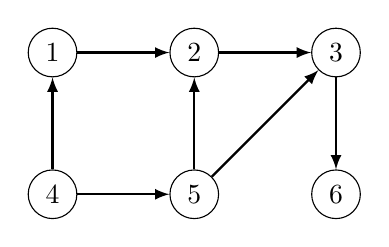
\begin{tikzpicture}[scale=0.9]
\node[draw, circle] (1) at (1,5) {$1$};
\node[draw, circle] (2) at (3,5) {$2$};
\node[draw, circle] (3) at (5,5) {$3$};
\node[draw, circle] (4) at (1,3) {$4$};
\node[draw, circle] (5) at (3,3) {$5$};
\node[draw, circle] (6) at (5,3) {$6$};

\path[draw,thick,->,>=latex] (1) -- (2);
\path[draw,thick,->,>=latex] (2) -- (3);
\path[draw,thick,->,>=latex] (4) -- (1);
\path[draw,thick,->,>=latex] (4) -- (5);
\path[draw,thick,->,>=latex] (5) -- (2);
\path[draw,thick,->,>=latex] (5) -- (3);
\path[draw,thick,->,>=latex] (3) -- (6);
\end{tikzpicture}
\end{center}
топологиялық сұрыпталған тізімі
$[4,1,5,2,3,6]$ осындай болады:
\begin{center}
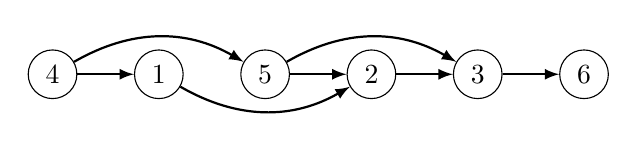
\begin{tikzpicture}[scale=0.9]
\node[draw, circle] (1) at (-6,0) {$1$};
\node[draw, circle] (2) at (-3,0) {$2$};
\node[draw, circle] (3) at (-1.5,0) {$3$};
\node[draw, circle] (4) at (-7.5,0) {$4$};
\node[draw, circle] (5) at (-4.5,0) {$5$};
\node[draw, circle] (6) at (-0,0) {$6$};

\path[draw,thick,->,>=latex] (1) edge [bend right=30] (2);
\path[draw,thick,->,>=latex] (2) -- (3);
\path[draw,thick,->,>=latex] (4) -- (1);
\path[draw,thick,->,>=latex] (4) edge [bend left=30] (5);
\path[draw,thick,->,>=latex] (5) -- (2);
\path[draw,thick,->,>=latex] (5) edge [bend left=30]  (3);
\path[draw,thick,->,>=latex] (3) -- (6);
\end{tikzpicture}
\end{center}

Циклсіз графты әрқашан топологиялық сұрыптауға болады.
Ал егер графта цикл болса, оны топологиялық сұрыптай алмаймыз. Себебі, циклдің бір төбесі циклдегі басқа төбеден
тізімде бұрын келе алмайды. 

Тереңдік бойынша іздеу бағытталған графта циклдардың бар-жоғын тексеруге де, ал цикл болмаған жағдайда топологиялық сұрыптауды құруға да мүмкіндік береді екен.

% An acyclic graph always has a topological sort.
% However, if the graph contains a cycle,
% it is not possible to form a topological sort,
% because no node of the cycle can appear
% before the other nodes of the cycle in the ordering.
% It turns out that depth-first search can be used
% to both check if a directed graph contains a cycle
% and, if it does not contain a cycle, to construct a topological sort.

\subsubsection{Алгоритм}

Алгоритмнің идеясы графтағы төбелерді 
бір-бірлеп өтуге, өту барысында төбенің бұрын қарастырылмағаны анықталса, 
сол төбеден тереңдігі бойынша ізденісті бастауға негізделеді.
Іздеу кезінде төбелердің үш түрлі күйі болады. Олар:

\begin{itemize}

\item 0-күй: төбе әлі қарастырылмаған (ақ)
\item 1-күй: төбе қарастыру барысында (сұрғылт)
\item 2-күй: төбе қарастырылды, яғни толық өңделді (қара сұр)
\end{itemize}

Басында әр төбе 0-күйіде болады. Кейін ізденіс төбеге бірінші рет жеткен кезде, ол 1-күйіге өтеді. Төбеден 
шығатын барлық төбелерін қарастырып болған кезде, ол 
2-күйге ауысады.
% Initially, the state of each node is 0.
% When a search reaches a node for the first time,
% its state becomes 1.
% Finally, after all successors of the node have
% been processed, its state becomes 2.

Егер графта цикл болса, біз оны іздеу процесінде табамыз. Өйткені ерте ме, кеш пе, 1-күйдегі төбеге бір қадаламыз.  Осы жағдайда топологиялық сұрыптау мүмкін болмай қалады.
% If the graph contains a cycle, we will find this out
% during the search, because sooner or later
% we will arrive at a node whose state is 1.
% In this case, it is not possible to construct a topological sort.

Егер графта цикл болмаса, біз графтағы төбелер 2-күйге
ауысқан кезде әр төбені тізімге қоса отырып, топологиялық сұрыптаймыз.

% If the graph does not contain a cycle, we can construct
% a topological sort by 
% adding each node to a list when the state of the node becomes 2.

\subsubsection{1-мысал}

Осы мысалда графтағы 1-ден 6-ға дейінгі төбелерді
өңдейміз:
% In the example graph, the search first proceeds
% from node 1 to node 6:

\begin{center}
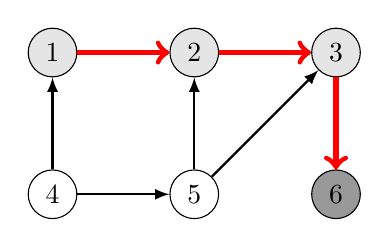
\begin{tikzpicture}[scale=0.9]
\node[draw, circle,fill=gray!20] (1) at (1,5) {$1$};
\node[draw, circle,fill=gray!20] (2) at (3,5) {$2$};
\node[draw, circle,fill=gray!20] (3) at (5,5) {$3$};
\node[draw, circle] (4) at (1,3) {$4$};
\node[draw, circle] (5) at (3,3) {$5$};
\node[draw, circle,fill=gray!80] (6) at (5,3) {$6$};

\path[draw,thick,->,>=latex] (4) -- (1);
\path[draw,thick,->,>=latex] (4) -- (5);
\path[draw,thick,->,>=latex] (5) -- (2);
\path[draw,thick,->,>=latex] (5) -- (3);
%\path[draw,thick,->,>=latex] (3) -- (6);

\path[draw=red,thick,->,line width=2pt] (1) -- (2);
\path[draw=red,thick,->,line width=2pt] (2) -- (3);
\path[draw=red,thick,->,line width=2pt] (3) -- (6);
\end{tikzpicture}
\end{center}

Алдымен 6-төбе өңделді, сондықтан оны тізімге қосамыз.
Содан кейін 3, 2 және 1-төбелерді де тізімге қосамыз:
% Now node 6 has been processed, so it is added to the list.
% After this, also nodes 3, 2 and 1 are added to the list:

\begin{center}
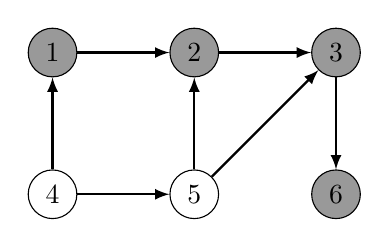
\begin{tikzpicture}[scale=0.9]
\node[draw, circle,fill=gray!80] (1) at (1,5) {$1$};
\node[draw, circle,fill=gray!80] (2) at (3,5) {$2$};
\node[draw, circle,fill=gray!80] (3) at (5,5) {$3$};
\node[draw, circle] (4) at (1,3) {$4$};
\node[draw, circle] (5) at (3,3) {$5$};
\node[draw, circle,fill=gray!80] (6) at (5,3) {$6$};

\path[draw,thick,->,>=latex] (1) -- (2);
\path[draw,thick,->,>=latex] (2) -- (3);
\path[draw,thick,->,>=latex] (4) -- (1);
\path[draw,thick,->,>=latex] (4) -- (5);
\path[draw,thick,->,>=latex] (5) -- (2);
\path[draw,thick,->,>=latex] (5) -- (3);
\path[draw,thick,->,>=latex] (3) -- (6);
\end{tikzpicture}
\end{center}

Қазіргі тізім -- $[6,3,2,1]$. Келесі ізденіс
4-төбеден басталады:
% At this point, the list is $[6,3,2,1]$.
% The next search begins at node 4:

\begin{center}
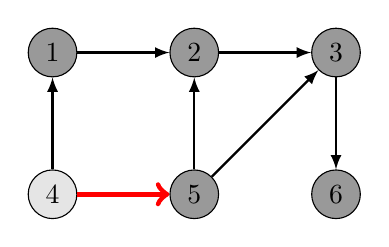
\begin{tikzpicture}[scale=0.9]
\node[draw, circle,fill=gray!80] (1) at (1,5) {$1$};
\node[draw, circle,fill=gray!80] (2) at (3,5) {$2$};
\node[draw, circle,fill=gray!80] (3) at (5,5) {$3$};
\node[draw, circle,fill=gray!20] (4) at (1,3) {$4$};
\node[draw, circle,fill=gray!80] (5) at (3,3) {$5$};
\node[draw, circle,fill=gray!80] (6) at (5,3) {$6$};

\path[draw,thick,->,>=latex] (1) -- (2);
\path[draw,thick,->,>=latex] (2) -- (3);
\path[draw,thick,->,>=latex] (4) -- (1);
%\path[draw,thick,->,>=latex] (4) -- (5);
\path[draw,thick,->,>=latex] (5) -- (2);
\path[draw,thick,->,>=latex] (5) -- (3);
\path[draw,thick,->,>=latex] (3) -- (6);

\path[draw=red,thick,->,line width=2pt] (4) -- (5);
\end{tikzpicture}
\end{center}

Түпкі тізім -- $[6,3,2,1,5,4]$.
Біз барлық төбелерді өтіп шықтық және оларды тізімге қостық.
Енді топологиялық сұрыптау тізімін табу үшін 
соңғы тізімді кері төңкеру керек. Осылайша берілген графтың
топологиялық сұрыптау тізімі -- $[4,5,1,2,3,6]$:
% Thus, the final list is $[6,3,2,1,5,4]$.
% We have processed all nodes, so a topological sort has
% been found.
% The topological sort is the reverse list
% $[4,5,1,2,3,6]$:

\begin{center}
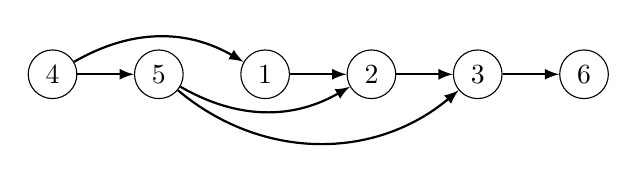
\begin{tikzpicture}[scale=0.9]
\node[draw, circle] (1) at (3,0) {$1$};
\node[draw, circle] (2) at (4.5,0) {$2$};
\node[draw, circle] (3) at (6,0) {$3$};
\node[draw, circle] (4) at (0,0) {$4$};
\node[draw, circle] (5) at (1.5,0) {$5$};
\node[draw, circle] (6) at (7.5,0) {$6$};

\path[draw,thick,->,>=latex] (1) -- (2);
\path[draw,thick,->,>=latex] (2) -- (3);
\path[draw,thick,->,>=latex] (4) edge [bend left=30] (1);
\path[draw,thick,->,>=latex] (4) -- (5);
\path[draw,thick,->,>=latex] (5) edge [bend right=30] (2);
\path[draw,thick,->,>=latex] (5) edge [bend right=40] (3);
\path[draw,thick,->,>=latex] (3) -- (6);
\end{tikzpicture}
\end{center}

Топологиялық сұрыптаудың бірегей еместігін және графта бірнеше топологиялық сұрыптаулар болуы мүмкін екенін ескергеніміз жөн.
% Note that a topological sort is not unique,
% and there can be several topological sorts for a graph.

\subsubsection{2-мысал}

Енді графта цикл болғандықтан топологиялық сұрыптауды
құра алмайтын мысалды қарастырайық:
% Let us now consider a graph for which we
% cannot construct a topological sort,
% because the graph contains a cycle:

\begin{center}
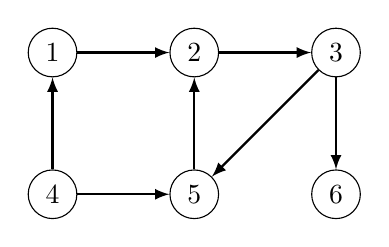
\begin{tikzpicture}[scale=0.9]
\node[draw, circle] (1) at (1,5) {$1$};
\node[draw, circle] (2) at (3,5) {$2$};
\node[draw, circle] (3) at (5,5) {$3$};
\node[draw, circle] (4) at (1,3) {$4$};
\node[draw, circle] (5) at (3,3) {$5$};
\node[draw, circle] (6) at (5,3) {$6$};

\path[draw,thick,->,>=latex] (1) -- (2);
\path[draw,thick,->,>=latex] (2) -- (3);
\path[draw,thick,->,>=latex] (4) -- (1);
\path[draw,thick,->,>=latex] (4) -- (5);
\path[draw,thick,->,>=latex] (5) -- (2);
\path[draw,thick,->,>=latex] (3) -- (5);
\path[draw,thick,->,>=latex] (3) -- (6);
\end{tikzpicture}
\end{center}
Ізденіс келесі төбелерді қарастырады:
% The search proceeds as follows:
\begin{center}
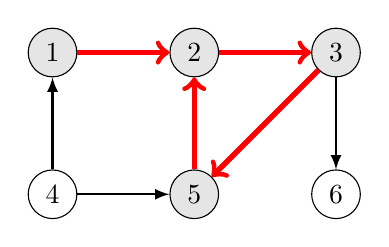
\begin{tikzpicture}[scale=0.9]
\node[draw, circle,fill=gray!20] (1) at (1,5) {$1$};
\node[draw, circle,fill=gray!20] (2) at (3,5) {$2$};
\node[draw, circle,fill=gray!20] (3) at (5,5) {$3$};
\node[draw, circle] (4) at (1,3) {$4$};
\node[draw, circle,fill=gray!20] (5) at (3,3) {$5$};
\node[draw, circle] (6) at (5,3) {$6$};

\path[draw,thick,->,>=latex] (4) -- (1);
\path[draw,thick,->,>=latex] (4) -- (5);
\path[draw,thick,->,>=latex] (3) -- (6);

\path[draw=red,thick,->,line width=2pt] (1) -- (2);
\path[draw=red,thick,->,line width=2pt] (2) -- (3);
\path[draw=red,thick,->,line width=2pt] (3) -- (5);
\path[draw=red,thick,->,line width=2pt] (5) -- (2);
\end{tikzpicture}
\end{center}
Ізденіс күйі 1-ге тең 2-төбеге жетеді. Бұл графтың циклды қамтитынын білдіреді. 
Бұл мысалда
$2 \rightarrow 3 \rightarrow 5 \rightarrow 2$ түріндегі цикл бар.
% The search reaches node 2 whose state is 1,
% which means that the graph contains a cycle.
% In this example, there is a cycle
% $2 \rightarrow 3 \rightarrow 5 \rightarrow 2$.

\section{Динамикалық бағдарламалау}

Егер бағытталған графта цикл болмаса,
оған динамикалық бағдарламалау әдісін қолдануға болады.
Мысалы, біз екі төбе арасындағы жолдарға қатысты
келесі мәселелерді тиімді шеше аламыз:
% If a directed graph is acyclic,
% dynamic programming can be applied to it.
% For example, we can efficiently solve the following
% problems concerning paths from a starting node
% to an ending node:

\begin{itemize}
\item қанша әртүрлі жол бар?
\item ең қысқа/ең ұзын жол қандай?
\item жолдағы қырлардың минималды/максималды саны қандай?
\item әр жолда қандай төбелер міндетті түрде кездеседі?
\end{itemize}

% \begin{itemize}
% \item how many different paths are there?
% \item what is the shortest/longest path?
% \item what is the minimum/maximum number of edges in a path?
% \item which nodes certainly appear in any path?
% \end{itemize}

\subsubsection{Жолдардың санын есептеу}
% \subsubsection{Counting the number of paths}

Мысалы, 1-төбеден 6-төбеге дейінгі жолдардың санын есептейік:
% As an example, let us calculate the number of paths
% from node 1 to node 6 in the following graph:

\begin{center}
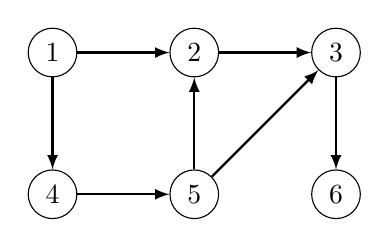
\begin{tikzpicture}[scale=0.9]
\node[draw, circle] (1) at (1,5) {$1$};
\node[draw, circle] (2) at (3,5) {$2$};
\node[draw, circle] (3) at (5,5) {$3$};
\node[draw, circle] (4) at (1,3) {$4$};
\node[draw, circle] (5) at (3,3) {$5$};
\node[draw, circle] (6) at (5,3) {$6$};

\path[draw,thick,->,>=latex] (1) -- (2);
\path[draw,thick,->,>=latex] (2) -- (3);
\path[draw,thick,->,>=latex] (1) -- (4);
\path[draw,thick,->,>=latex] (4) -- (5);
\path[draw,thick,->,>=latex] (5) -- (2);
\path[draw,thick,->,>=latex] (5) -- (3);
\path[draw,thick,->,>=latex] (3) -- (6);
\end{tikzpicture}
\end{center}
Төмендегідей үш жол бар:
% There are a total of three such paths:
\begin{itemize}
\item $1 \rightarrow 2 \rightarrow 3 \rightarrow 6$
\item $1 \rightarrow 4 \rightarrow 5 \rightarrow 2 \rightarrow 3 \rightarrow 6$
\item $1 \rightarrow 4 \rightarrow 5 \rightarrow 3 \rightarrow 6$
\end{itemize}

Біз 1-төбеден басталып $x$-төбеде аяқталатын жолдардын санын
$\texttt{paths}(x)$ деп белгілейік.
Ең басында $\texttt{paths}(1)=1$ тең болады.
Кейін $\texttt{paths}(x)$ жиымының басқа мәндерін есептеу
үшін рекурсия қолдана аламыз.
% As a base case, $\texttt{paths}(1)=1$.
% Then, to calculate other values of $\texttt{paths}(x)$,
% we may use the recursion.
\[\texttt{paths}(x) = \texttt{paths}(a_1)+\texttt{paths}(a_2)+\cdots+\texttt{paths}(a_k)\]
бұл жерде $a_1,a_2,\ldots,a_k$ деп $x$-төбемен көршілес төбелер
белгіленген.
% where $a_1,a_2,\ldots,a_k$ are the nodes from which there
% is an edge to $x$.
Граф ациклді болғандықтан $\texttt{paths}(x)$ жиымның мәндерін
топологиялық сұрыптау тізімінің ретімен есептеп шығуға болады.
Жоғарыдағы графтың топологиялық сұрыпталған тізімі:
% Since the graph is acyclic, the values of $\texttt{paths}(x)$
% can be calculated in the order of a topological sort.
% A topological sort for the above graph is as follows:
\begin{center}
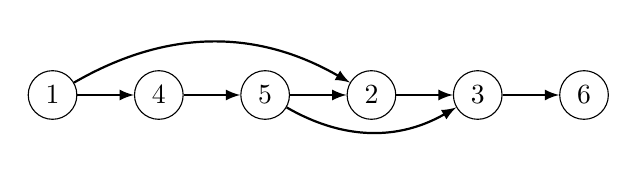
\begin{tikzpicture}[scale=0.9]
\node[draw, circle] (1) at (0,0) {$1$};
\node[draw, circle] (2) at (4.5,0) {$2$};
\node[draw, circle] (3) at (6,0) {$3$};
\node[draw, circle] (4) at (1.5,0) {$4$};
\node[draw, circle] (5) at (3,0) {$5$};
\node[draw, circle] (6) at (7.5,0) {$6$};

\path[draw,thick,->,>=latex] (1) edge [bend left=30] (2);
\path[draw,thick,->,>=latex] (2) -- (3);
\path[draw,thick,->,>=latex] (1) -- (4);
\path[draw,thick,->,>=latex] (4) -- (5);
\path[draw,thick,->,>=latex] (5) -- (2);
\path[draw,thick,->,>=latex] (5) edge [bend right=30] (3);
\path[draw,thick,->,>=latex] (3) -- (6);
\end{tikzpicture}
\end{center}
Сондықтан жолдардың саны төмендегідей болады:
% Hence, the numbers of paths are as follows:
\begin{center}
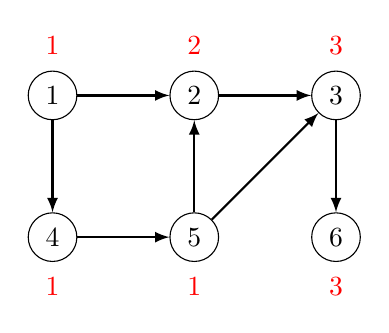
\begin{tikzpicture}[scale=0.9]
\node[draw, circle] (1) at (1,5) {$1$};
\node[draw, circle] (2) at (3,5) {$2$};
\node[draw, circle] (3) at (5,5) {$3$};
\node[draw, circle] (4) at (1,3) {$4$};
\node[draw, circle] (5) at (3,3) {$5$};
\node[draw, circle] (6) at (5,3) {$6$};

\path[draw,thick,->,>=latex] (1) -- (2);
\path[draw,thick,->,>=latex] (2) -- (3);
\path[draw,thick,->,>=latex] (1) -- (4);
\path[draw,thick,->,>=latex] (4) -- (5);
\path[draw,thick,->,>=latex] (5) -- (2);
\path[draw,thick,->,>=latex] (5) -- (3);
\path[draw,thick,->,>=latex] (3) -- (6);

\node[color=red] at (1,2.3) {$1$};
\node[color=red] at (3,2.3) {$1$};
\node[color=red] at (5,2.3) {$3$};
\node[color=red] at (1,5.7) {$1$};
\node[color=red] at (3,5.7) {$2$};
\node[color=red] at (5,5.7) {$3$};
\end{tikzpicture}
\end{center}

Мысалы, $\texttt{paths}(3)$ мәнін есептеу үшін біз 
$\texttt{paths}(2)+\texttt{paths}(5)$ формуласын қолдана аламыз.
Себебі 2 және 5 төбелерінен 3-төбеге қыр бар.
Мұндағы $\texttt{paths}(2)=2$ және $\texttt{paths}(5)=1$ тең болғандықтан,
біз $\texttt{paths}(3)=3$ мәнін осылай қорытындылаймыз.

% For example, to calculate the value of $\texttt{paths}(3)$,
% we can use the formula $\texttt{paths}(2)+\texttt{paths}(5)$,
% because there are edges from nodes 2 and 5
% to node 3.
% Since $\texttt{paths}(2)=2$ and $\texttt{paths}(5)=1$, we conclude that $\texttt{paths}(3)=3$.

\subsubsection{Дейкстра алгоритмін кеңейту}

\index{Дейкстра алгоритмі}

Бастапқы төбеден қалған төбелерге мейлінше қысқа жолмен жетудің мүмкін тәсілдерін көрсететін бағытталған, ациклді граф Дейкстра алгоритмінің жанама өніміне жатады. 
Бұл жаңа граф төбелерге бару үшін қолданылатын қырларды қалдырып, қалған қолданбайтын
қырларды алып тастау арқылы құрылады. Яғни бастапқы төбеден түпнұсқа графтағы әр
төбеге баратын ең қысқа жолдардың қырларын тауып, тек соларды қалдырады.
% A by-product of Dijkstra's algorithm is a directed, acyclic
% graph that indicates for each node of the original graph
% the possible ways to reach the node using a shortest path
% from the starting node.
Динамикалық бағдарламалауды сол жаңа графқа қолдануға болады.
% Dynamic programming can be applied to that graph.
Мысалы, төмендегі графта
% For example, in the graph
\begin{center}
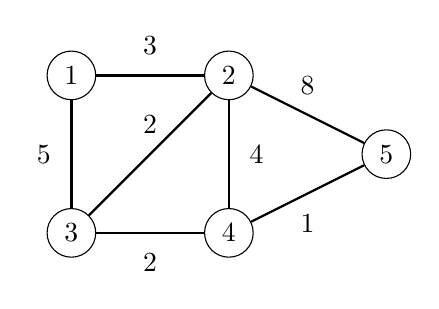
\begin{tikzpicture}
\node[draw, circle] (1) at (0,0) {$1$};
\node[draw, circle] (2) at (2,0) {$2$};
\node[draw, circle] (3) at (0,-2) {$3$};
\node[draw, circle] (4) at (2,-2) {$4$};
\node[draw, circle] (5) at (4,-1) {$5$};

\path[draw,thick,-] (1) -- node[font=\small,label=above:3] {} (2);
\path[draw,thick,-] (1) -- node[font=\small,label=left:5] {} (3);
\path[draw,thick,-] (2) -- node[font=\small,label=right:4] {} (4);
\path[draw,thick,-] (2) -- node[font=\small,label=above:8] {} (5);
\path[draw,thick,-] (3) -- node[font=\small,label=below:2] {} (4);
\path[draw,thick,-] (4) -- node[font=\small,label=below:1] {} (5);
\path[draw,thick,-] (2) -- node[font=\small,label=above:2] {} (3);
\end{tikzpicture}
\end{center}
1-төбеден шығатын ең қысқа жолдар келесі қырларды қолданады:
% the shortest paths from node 1 may use the following edges:
\begin{center}
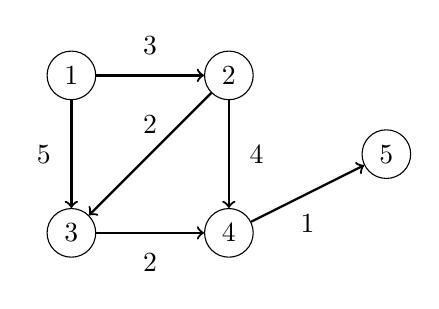
\begin{tikzpicture}
\node[draw, circle] (1) at (0,0) {$1$};
\node[draw, circle] (2) at (2,0) {$2$};
\node[draw, circle] (3) at (0,-2) {$3$};
\node[draw, circle] (4) at (2,-2) {$4$};
\node[draw, circle] (5) at (4,-1) {$5$};

\path[draw,thick,->] (1) -- node[font=\small,label=above:3] {} (2);
\path[draw,thick,->] (1) -- node[font=\small,label=left:5] {} (3);
\path[draw,thick,->] (2) -- node[font=\small,label=right:4] {} (4);
\path[draw,thick,->] (3) -- node[font=\small,label=below:2] {} (4);
\path[draw,thick,->] (4) -- node[font=\small,label=below:1] {} (5);
\path[draw,thick,->] (2) -- node[font=\small,label=above:2] {} (3);
\end{tikzpicture}
\end{center}

Мысалы, біз динамикалық бағдарламалау арқылы 
1-төбеден 5-төбеге дейінгі жолдардың санын таба аламыз:
% Now we can, for example, calculate the number of
% shortest paths from node 1 to node 5
% using dynamic programming:
\begin{center}
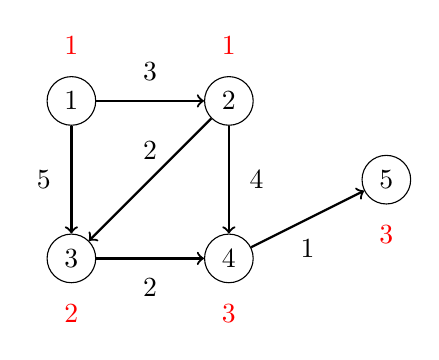
\begin{tikzpicture}
\node[draw, circle] (1) at (0,0) {$1$};
\node[draw, circle] (2) at (2,0) {$2$};
\node[draw, circle] (3) at (0,-2) {$3$};
\node[draw, circle] (4) at (2,-2) {$4$};
\node[draw, circle] (5) at (4,-1) {$5$};

\path[draw,thick,->] (1) -- node[font=\small,label=above:3] {} (2);
\path[draw,thick,->] (1) -- node[font=\small,label=left:5] {} (3);
\path[draw,thick,->] (2) -- node[font=\small,label=right:4] {} (4);
\path[draw,thick,->] (3) -- node[font=\small,label=below:2] {} (4);
\path[draw,thick,->] (4) -- node[font=\small,label=below:1] {} (5);
\path[draw,thick,->] (2) -- node[font=\small,label=above:2] {} (3);

\node[color=red] at (0,0.7) {$1$};
\node[color=red] at (2,0.7) {$1$};
\node[color=red] at (0,-2.7) {$2$};
\node[color=red] at (2,-2.7) {$3$};
\node[color=red] at (4,-1.7) {$3$};
\end{tikzpicture}
\end{center}

\subsubsection{Есептерді граф тәріздес қарастыру}

Шынында кез келген динамикалық бағдарламалау есебін бағытталған,
ациклді граф тәрізді қарастыруға болады. 
Мұндай графта әрбір төбе динамикалық бағдарламалау 
мәніне сәйкес келеді және қырлар мәндердің бір-біріне
тәуелділігін көрсетеді.
% Actually, any dynamic programming problem
% can be represented as a directed, acyclic graph.
% In such a graph, each node corresponds to a dynamic programming state
% and the edges indicate how the states depend on each other.

Мысалы, $\{c_1,c_2,\ldots,c_k\}$ тиындарын қолдану арқылы
қосындысы $n$ болатын есепті қарастырайық.
Бұл есепті шығару үшін граф қолдана аламыз.
Графта әр төбе тиындардың қосындысын белгілейді және 
қырлар қандай тиындар таңдау керек екенін белгілейді.
Мысалы, $\{1,3,4\}$ тиындары бар және $n=6$ тең болатын графтың
көрінісі осындай болады:
% As an example, consider the problem
% of forming a sum of money $n$
% using coins
% $\{c_1,c_2,\ldots,c_k\}$.
% In this problem, we can construct a graph where
% each node corresponds to a sum of money,
% and the edges show how the coins can be chosen.
% For example, for coins $\{1,3,4\}$ and $n=6$,
% the graph is as follows:
\begin{center}
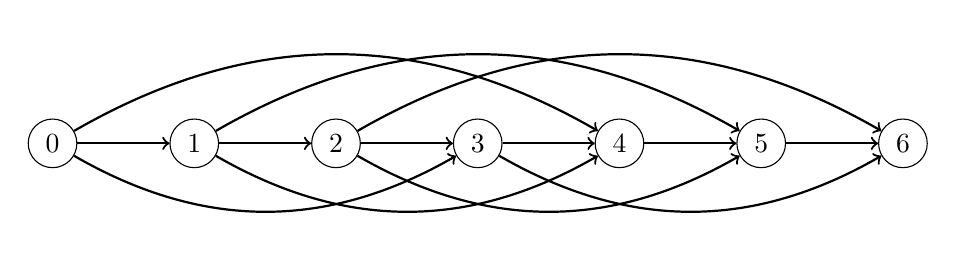
\begin{tikzpicture}[scale=0.9]
\node[draw, circle] (0) at (0,0) {$0$};
\node[draw, circle] (1) at (2,0) {$1$};
\node[draw, circle] (2) at (4,0) {$2$};
\node[draw, circle] (3) at (6,0) {$3$};
\node[draw, circle] (4) at (8,0) {$4$};
\node[draw, circle] (5) at (10,0) {$5$};
\node[draw, circle] (6) at (12,0) {$6$};

\path[draw,thick,->] (0) -- (1);
\path[draw,thick,->] (1) -- (2);
\path[draw,thick,->] (2) -- (3);
\path[draw,thick,->] (3) -- (4);
\path[draw,thick,->] (4) -- (5);
\path[draw,thick,->] (5) -- (6);

\path[draw,thick,->] (0) edge [bend right=30] (3);
\path[draw,thick,->] (1) edge [bend right=30] (4);
\path[draw,thick,->] (2) edge [bend right=30] (5);
\path[draw,thick,->] (3) edge [bend right=30] (6);

\path[draw,thick,->] (0) edge [bend left=30] (4);
\path[draw,thick,->] (1) edge [bend left=30] (5);
\path[draw,thick,->] (2) edge [bend left=30] (6);
\end{tikzpicture}
\end{center}

% Осы көрініс арқылы 0-төбеден $n$-төбеге дейін
% жетудің жолдарын көрсетеді, яғни біз тек 1 тиындарын алып
% 6 сомасын құра аламыз. Сондай-ақ бастапқыда 4 тиынын алып, кейін екі 1
% тиындарын алуға болады. 
Біз графтағы 0-төбеден $n$-төбеге дейінгі ең қысқа жолды табу арқылы $n$ сомасын
құрайтын минималды тиындар санын таба аламыз. Осы мысалда 0-ден
3-төбеге, содан соң 6-төбеге дейінгі жол ең қысқа жол болып табылады. Бұл
жерде тек екі қыр қолданылған. Сонда 6 сомасын құру үшін 
минималды тиындар саны екі болмақ. Одан басқа, қарастырылған граф бізге
0-төбеден $n$-төбеге дейінгі жолдардың санын табу арқылы 
$n$ суммасына жететін шешімдердің санын табуға көмектеседі.

% I extended it because I think it is necessary.
% Using this representation,
% the shortest path from node 0 to node $n$
% corresponds to a solution with the minimum number of coins,
% and the total number of paths from node 0 to node $n$
% equals the total number of solutions.

\section{Мирасқорлар графы}

\index{мирасқорлар графы}
\index{функционалды граф}

Тараудың қалған бөлігінде біз \key{мирасқорлар графына} (successor graph) тоқталамыз.
Бұл графтарда әр төбенің шығыстың жарты дәрежесі дәрежесі 1-ге тең, яғни әр төбеден
тек бір ғана қыр шығады.
Мирасқорлар графы бір немесе бірнеше компоненттерден тұрады.
Ал компоненттер бір циклды және оған бағытталған бірнеше жолдарды қамтиды.
% For the rest of the chapter,
% we will focus on \key{successor graphs}.
% In those graphs,
% the outdegree of each node is 1, i.e.,
% exactly one edge starts at each node.
% A successor graph consists of one or more
% components, each of which contains
% one cycle and some paths that lead to it.

Мирасқорлар графтарын кейде функционалды граф деп те
атайды. Себебі кез келген мирасқорлар графы графтағы
қырларды анықтайтын функцияға сәйкес келеді. 
Функцияның параметрі графтың төбесі болса,
оның мәні мирасқор төбеге сәйкес келеді.
% Successor graphs are sometimes called
% \key{functional graphs}.
% The reason for this is that any successor graph
% corresponds to a function that defines
% the edges of the graph.
% The parameter for the function is a node of the graph,
% and the function gives the successor of that node.

Мысалы, төмендегі функциямен
\begin{center}
\begin{tabular}{r|rrrrrrrrr}
$x$ & 1 & 2 & 3 & 4 & 5 & 6 & 7 & 8 & 9 \\
\hline
$\texttt{succ}(x)$ & 3 & 5 & 7 & 6 & 2 & 2 & 1 & 6 & 3 \\
\end{tabular}
\end{center}
келесі графты құруға болады:
\begin{center}
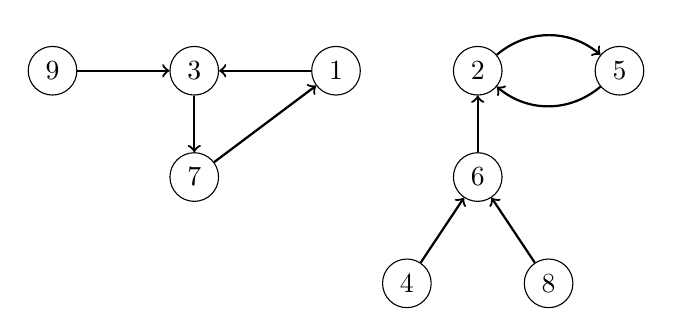
\begin{tikzpicture}[scale=0.9]
\node[draw, circle] (1) at (0,0) {$1$};
\node[draw, circle] (2) at (2,0) {$2$};
\node[draw, circle] (3) at (-2,0) {$3$};
\node[draw, circle] (4) at (1,-3) {$4$};
\node[draw, circle] (5) at (4,0) {$5$};
\node[draw, circle] (6) at (2,-1.5) {$6$};
\node[draw, circle] (7) at (-2,-1.5) {$7$};
\node[draw, circle] (8) at (3,-3) {$8$};
\node[draw, circle] (9) at (-4,0) {$9$};

\path[draw,thick,->] (1) -- (3);
\path[draw,thick,->] (2)  edge [bend left=40] (5);
\path[draw,thick,->] (3) -- (7);
\path[draw,thick,->] (4) -- (6);
\path[draw,thick,->] (5)  edge [bend left=40] (2);
\path[draw,thick,->] (6) -- (2);
\path[draw,thick,->] (7) -- (1);
\path[draw,thick,->] (8) -- (6);
\path[draw,thick,->] (9) -- (3);
\end{tikzpicture}
\end{center}

Мирасқорлар графындағы әр төбеде өзінің белгілі және бірегей
мирасқоры болғандықтан, біз $\texttt{succ}(x,k)$ функциясын
жария ете аламыз. Функция бізге $x$ төбесінен бастап, алға $k$ қадам жасау арқылы жететін төбені береді.
Мысалы, жоғарыдағы графта $\texttt{succ}(4,6)=2$ тең.
Себебі біз 2-төбеге 4-төбеден 6 қадам жасау арқылы жетеміз.
% Since each node of a successor graph has a
% unique successor, we can also define a function $\texttt{succ}(x,k)$
% that gives the node that we will reach if
% we begin at node $x$ and walk $k$ steps forward.
% For example, in the above graph $\texttt{succ}(4,6)=2$,
% because we will reach node 2 by walking 6 steps from node 4:

\begin{center}
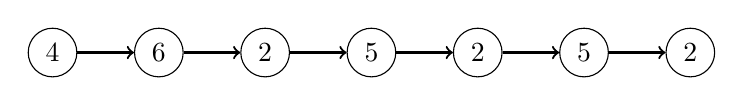
\begin{tikzpicture}[scale=0.9]
\node[draw, circle] (1) at (0,0) {$4$};
\node[draw, circle] (2) at (1.5,0) {$6$};
\node[draw, circle] (3) at (3,0) {$2$};
\node[draw, circle] (4) at (4.5,0) {$5$};
\node[draw, circle] (5) at (6,0) {$2$};
\node[draw, circle] (6) at (7.5,0) {$5$};
\node[draw, circle] (7) at (9,0) {$2$};

\path[draw,thick,->] (1) -- (2);
\path[draw,thick,->] (2) -- (3);
\path[draw,thick,->] (3) -- (4);
\path[draw,thick,->] (4) -- (5);
\path[draw,thick,->] (5) -- (6);
\path[draw,thick,->] (6) -- (7);
\end{tikzpicture}
\end{center}

$\texttt{succ}(x,k)$ мәнін есептеудің қарапайым жолы
$x$ төбесінен басталып, $k$ қадам алға жүру. Бұл $O(k)$ уақыт алады.
Дегенмен алдын ала өңдеу арқылы $\texttt{succ}(x,k)$-тың әр мәнін
$O(\log k)$ уақытта табуға болады.
% A straightforward way to calculate a value of $\texttt{succ}(x,k)$
% is to start at node $x$ and walk $k$ steps forward, which takes $O(k)$ time.
% However, using preprocessing, any value of $\texttt{succ}(x,k)$
% can be calculated in only $O(\log k)$ time.


Бұл жердегі идея екінің $k$ дәрежесі $u$ - дан басым болмайтындай $\texttt{succ}(x,k)$ - ның барлық мәндерін алдын ала есептеуге негізделеді. 

Келесі рекурсияны 
пайдалана отырып, мұны тиімді орындауға болады:
% The idea is to precalculate all values of $\texttt{succ}(x,k)$ where
% $k$ is a power of two and at most $u$, where $u$ is
% the maximum number of steps we will ever walk.
% This can be efficiently done, because
% we can use the following recursion:

\begin{equation*}
    \texttt{succ}(x,k) = \begin{cases}
               \texttt{succ}(x)              & k = 1\\
               \texttt{succ}(\texttt{succ}(x,k/2),k/2)   & k > 1\\
           \end{cases}
\end{equation*}

Мәндерді алдын ала өңдеу $O(n \log u)$ уақыт алады.
Себебі әр төбеге $O(\log u)$ мән есептеледі.
Жоғары графтағы бірінші мәндер:
% Precalculating the values takes $O(n \log u)$ time,
% because $O(\log u)$ values are calculated for each node.
% In the above graph, the first values are as follows:

\begin{center}
\begin{tabular}{r|rrrrrrrrr}
$x$ & 1 & 2 & 3 & 4 & 5 & 6 & 7 & 8 & 9 \\
\hline
$\texttt{succ}(x,1)$ & 3 & 5 & 7 & 6 & 2 & 2 & 1 & 6 & 3 \\
$\texttt{succ}(x,2)$ & 7 & 2 & 1 & 2 & 5 & 5 & 3 & 2 & 7 \\
$\texttt{succ}(x,4)$ & 3 & 2 & 7 & 2 & 5 & 5 & 1 & 2 & 3 \\
$\texttt{succ}(x,8)$ & 7 & 2 & 1 & 2 & 5 & 5 & 3 & 2 & 7 \\
$\cdots$ \\
\end{tabular}
\end{center}

Осы алдын ала есептеуден кейін $\texttt{succ}(x,k)$ - ның кез келген мәнін $k$ - ны екі дәрежелі қосындыларға жіктеу арқылы табуға болады. Мысалы, егер біз 
$\texttt{succ}(x,11)$ мәнін тапқымыз келсе, алдымен 11-ді $11=8+2+1$ түрінде жіктейміз.
Осыны қолдана отырып,
\[\texttt{succ}(x,11)=\texttt{succ}(\texttt{succ}(\texttt{succ}(x,8),2),1).\]
Мысалға бұрынғы графта: 
\[\texttt{succ}(4,11)=\texttt{succ}(\texttt{succ}(\texttt{succ}(4,8),2),1)=5.\]
% After this, any value of $\texttt{succ}(x,k)$ can be calculated
% by presenting the number of steps $k$ as a sum of powers of two.
% For example, if we want to calculate the value of $\texttt{succ}(x,11)$,
% we first form the representation $11=8+2+1$.
% Using that,
% \[\texttt{succ}(x,11)=\texttt{succ}(\texttt{succ}(\texttt{succ}(x,8),2),1).\]
% For example, in the previous graph
% \[\texttt{succ}(4,11)=\texttt{succ}(\texttt{succ}(\texttt{succ}(4,8),2),1)=5.\]

Осындай көрініс әрқашан да $O(\log k)$ қадамнан тұрады.
Сондықтан $\texttt{succ}(x,k)$ мәнін есептеу $O(\log k)$
уақыт алады.
% Such a representation always consists of
% $O(\log k)$ parts, so calculating a value of $\texttt{succ}(x,k)$
% takes $O(\log k)$ time.

\section{Циклді анықтау}

\index{цикл}
\index{циклді анықтау}

Циклға апаратын жолдан ғана тұратын мирасқорлар графын қарастырайық.
''Егер біз жүрісті бастапқы төбеден бастасақ, циклдегі бірінші
төбе қандай болады және цикл қанша төбелерді қамтиды?'' - деген сұрақ қоя аламыз. 
% Consider a successor graph that only contains
% a path that ends in a cycle.
% We may ask the following questions:
% if we begin our walk at the starting node,
% what is the first node in the cycle
% and how many nodes does the cycle contain?

Мысалы, төмендегі графта
% For example, in the graph

\begin{center}
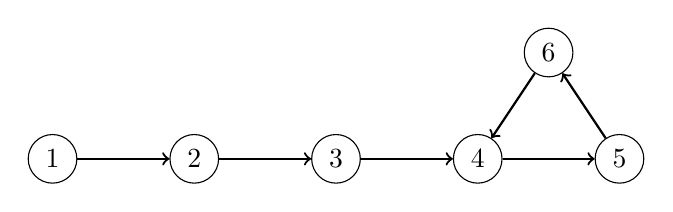
\begin{tikzpicture}[scale=0.9]
\node[draw, circle] (5) at (0,0) {$5$};
\node[draw, circle] (4) at (-2,0) {$4$};
\node[draw, circle] (6) at (-1,1.5) {$6$};
\node[draw, circle] (3) at (-4,0) {$3$};
\node[draw, circle] (2) at (-6,0) {$2$};
\node[draw, circle] (1) at (-8,0) {$1$};

\path[draw,thick,->] (1) -- (2);
\path[draw,thick,->] (2) -- (3);
\path[draw,thick,->] (3) -- (4);
\path[draw,thick,->] (4) -- (5);
\path[draw,thick,->] (5) -- (6);
\path[draw,thick,->] (6) -- (4);
\end{tikzpicture}
\end{center}
біз жүрісті 1-төбеден бастаймыз.
Циклге жататын бірінші төбе ол 4 және цикл 3 (4, 5 және 6)
төбелерден тұрады.
% we begin our walk at node 1,
% the first node that belongs to the cycle is node 4, and the cycle consists
% of three nodes (4, 5 and 6).

Циклді табудың оңай жолына графты өтіп шығу және жеткен
барлық төбелерді қадағалау жатады. Бір төбеге екінші рет жеткенде
біз төбе циклдің бірінші төбесі екенін қорыта аламыз.
Осы әдіс $O(n)$ уақытында жұмыс істейді және $O(n)$ жадысын қолданады.
% A simple way to detect the cycle is to walk in the
% graph and keep track of
% all nodes that have been visited. Once a node is visited
% for the second time, we can conclude
% that the node is the first node in the cycle.
% This method works in $O(n)$ time and also uses
% $O(n)$ memory.

Дегенмен циклді анықтауға арналған жақсырақ алгоритмдер де бар.
Олардың уақытша тиімділігі $O(n)$ болып қалады, бірақ
$O(1)$ жадысын ғана қолданады. Графта $n$ үлкен болса, бұл алгоритмнің елеулі жақсарғанын байқатады.
Әрі қарай біз осы қасиеттерге қол жеткізетін Флойд алгоритмін талқылаймыз.
% However, there are better algorithms for cycle detection.
% The time complexity of such algorithms is still $O(n)$,
% but they only use $O(1)$ memory. 
% This is an important improvement if $n$ is large.
% Next we will discuss Floyd's algorithm that
% achieves these properties.

\subsubsection{Флойд алгоритмі}

\index{Флойд алгоритмі}

\key{Флойд алгоритмі}\footnote{Алгоритм идеясын Р.В.Флойдқа телиді \cite{knu982}, дегенмен алгоритмді шынымен Флойдтың   ашқаны белгісіз.}
графта $a$ және $b$ нұсқағыштары арқылы жылжиды. Екі нұсқағыш та
жүрісті $x$ төбесінен бастайды. Кейін әр қадамда $a$ нұсқағышы
бір қадам алдыға жылжиды, ал $b$ екі қадам алдыға жылжиды. Осы үдеріс
екі нұсқағыштар бір-бірімен кездескенге дейін жалғасады:
% walks forward 
% in the graph using two pointers $a$ and $b$.
% Both pointers begin at a node $x$ that
% is the starting node of the graph.
% Then, on each turn, the pointer $a$ walks
% one step forward and the pointer $b$
% walks two steps forward.
% The process continues until
% the pointers meet each other:
\begin{lstlisting}
a = succ(x);
b = succ(succ(x));
while (a != b) {
    a = succ(a);
    b = succ(succ(b));
}
\end{lstlisting}

Осы сәтте $a$ нұсқағышы $k$ қадам жүреді, ал $b$ нұсқағышы
$2k$ қадам жүреді. Сондықтан циклдің ұзындығы $k$-ға  бөлінеді. Енді
циклге жататын бірінші төбені табу үшін $a$ нұсқағышын $x$-төбеге қойып,
қайтадан нұсқағыштарды кездескенге дейін біртіндеп жылжыту қажет.

% At this point, the pointer $a$ has walked $k$ steps
% and the pointer $b$ has walked $2k$ steps,
% so the length of the cycle divides $k$.
% Thus, the first node that belongs to the cycle
% can be found by moving the pointer $a$ to node $x$
% and advancing the pointers
% step by step until they meet again.
\begin{lstlisting}
a = x;
while (a != b) {
    a = succ(a);
    b = succ(b);
}
first = a;
\end{lstlisting}

Содан кейін циклдің ұзындығын төмендегідей етіп табуға болады:
% After this, the length of the cycle
% can be calculated as follows:
\begin{lstlisting}
b = succ(a);
length = 1;
while (a != b) {
    b = succ(b);
    length++;
}
\end{lstlisting}
